\documentclass[aspectratio=169]{beamer}
\usepackage{graphicx}
\usepackage{listings}
\lstset{
    basicstyle=\ttfamily
}

\usepackage{hyperref}

\usetheme{metropolis}
\title{Quantified Tasks}
\institute{Engineers for Exploration, UC San Diego}
\logo{
\includegraphics[height=0.62cm,keepaspectratio]{e4e_logo_350x136.png}}
\setbeamertemplate{caption}[numbered]

\begin{document}
\maketitle
\begin{frame}{Obligatory XKCD}
    \centering
    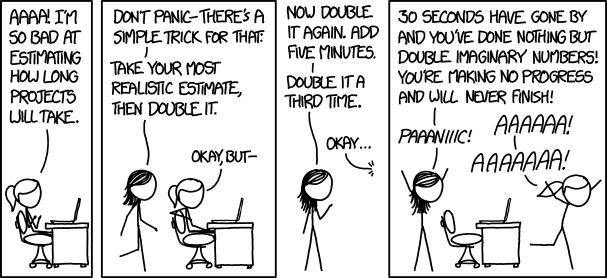
\includegraphics[width=\textwidth,height=0.7\textheight,keepaspectratio]{xkcd_1658.png} \footnote{\url{https://xkcd.com/1658/}}
\end{frame}
\begin{frame}{Fundamentals: What do we need to plan?}
    \begin{itemize}
        \item What do we need to accomplish?
        \item How long is that going to take?
    \end{itemize}
\end{frame}
\begin{frame}{The Church of Agile}
    \centering
    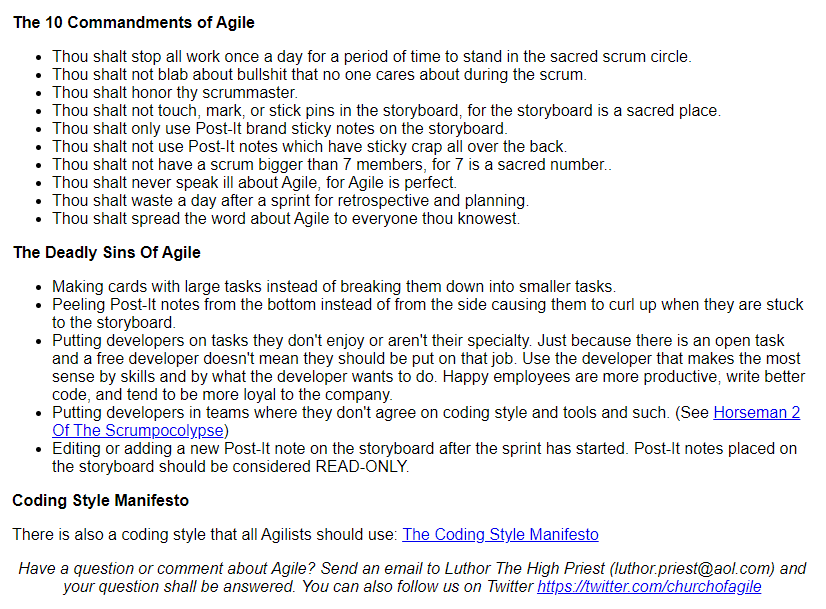
\includegraphics[width=\textwidth,height=0.8\textheight,keepaspectratio]{church_of_agile_10_commandments.png} \footnote{\url{https://www.thechurchofagile.org/commandments.php}}
\end{frame}
\begin{frame}{Agile: Story Points}
    \centering
    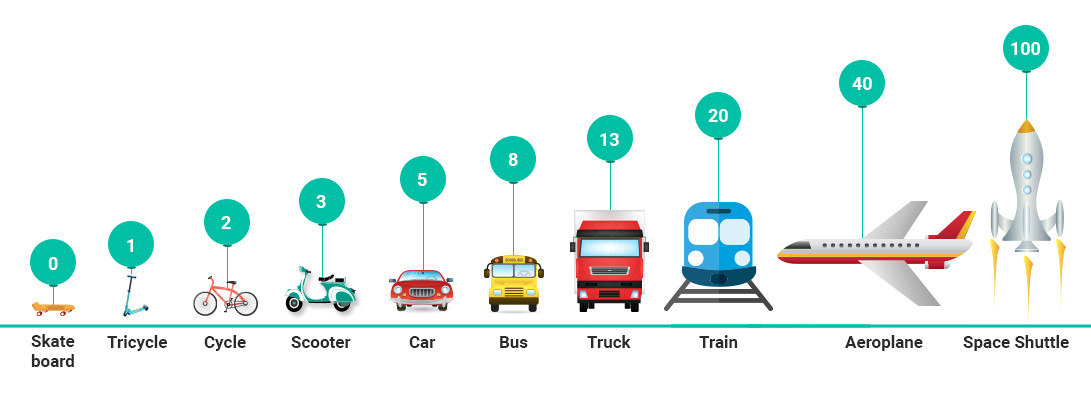
\includegraphics[width=\textwidth,height=0.8\textheight,keepaspectratio]{agile_story_points.jpg} \footnote{\url{https://www.linkedin.com/pulse/understanding-agile-story-points-suren-gaur}}
\end{frame}
\begin{frame}{Exercise \#1}
    Let's define making eggs and bacon as 3 story points.

    How many story points is making a hamburger?
\end{frame}
\begin{frame}{Exercise \#1}
    How about making Beef Wellington?
\end{frame}
\begin{frame}{Agile: Story Points}
    \centering
    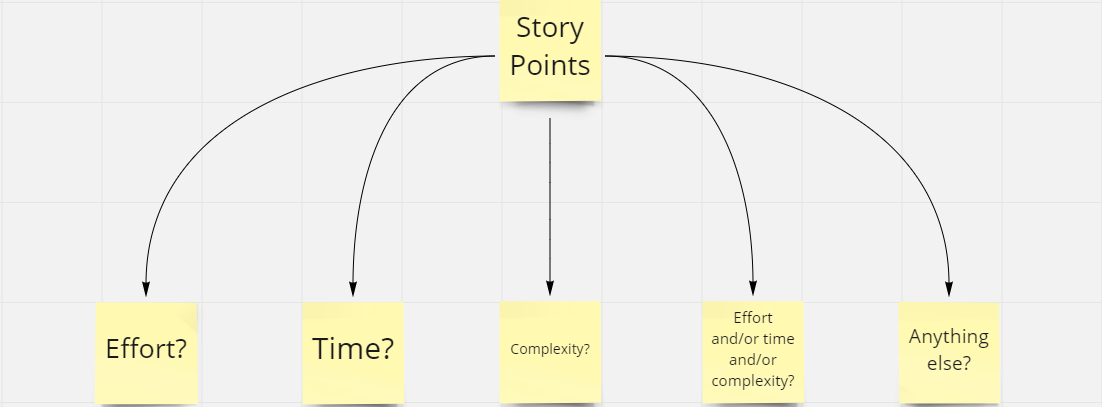
\includegraphics[width=\textwidth,height=0.8\textheight,keepaspectratio]{story_points_meaningless.png} \footnote{\url{https://maciejjarosz.medium.com/the-conundrum-about-story-points-pointless-or-not-b5d715180c96}}
\end{frame}
\begin{frame}{What do we actually want to know?}
    \begin{itemize}
        \item Planning
        \begin{itemize}
            \item Impact
            \item Gravity
            \item Priority
        \end{itemize}
        \item Estimation
        \begin{itemize}
            \item Distance
            \item Friction
            \item Relativity
        \end{itemize}
        \item Stability
        \begin{itemize}
            \item Origin
            \item Caught
        \end{itemize}
    \end{itemize}
    See \url{https://www.quantifiedtasks.org/p/overview}
\end{frame}
\section{Planning Measures}
\begin{frame}{Impact}
    \begin{itemize}
        \item Importance of Task to goals of the Solution
        \item 1 - Wishlist
        \item 5 - Essential
        \item Defined by product owner/stakeholders
    \end{itemize}
\end{frame}
\begin{frame}{Gravity}
    \begin{itemize}
        \item Importance of Task to the next release
        \item 1 - Not slated for inclusion
        \item 5 - Must-have
        \item Defined by product owner/stakeholders/developers
    \end{itemize}
\end{frame}
\begin{frame}{Priority}
    \begin{itemize}
        \item Urgency of Task
        \item 1 - Not on the schedule
        \item 4 - Now
        \item 5 - Emergency!
        \item Defined by product owner/developers
    \end{itemize}
\end{frame}
\section{Estimation Measures}
\begin{frame}{Distance}
    \begin{itemize}
        \item Estimated time frame for completion
        \item \textbf{Time frame if you understood everything about the task}
        \item 1 - Single work session
        \item 5 - Exceed a sprint
    \end{itemize}
\end{frame}
\begin{frame}{Friction}
    \begin{itemize}
        \item Available documentation and precedent for Task
        \item 1 - Complete tutorial available (i.e. follow the tutorial)
        \item 5 - Pure invention
    \end{itemize}
\end{frame}
\begin{frame}{Relativity}
    \begin{itemize}
        \item Likelihood that the task is a ``black hole'' with an indeterminable completion date
        \item 1 - No known uncertainty (i.e. no schedule risk)
        \item 5 - Virtually no certainty (i.e. extreme schedule risk)
    \end{itemize}
\end{frame}
\begin{frame}{Energy Points}
    $$(Distance + Friction) \times Relativity$$
\end{frame}
\section{Stability Measures}
\begin{frame}{Software Development Lifecycle}
    \centering
    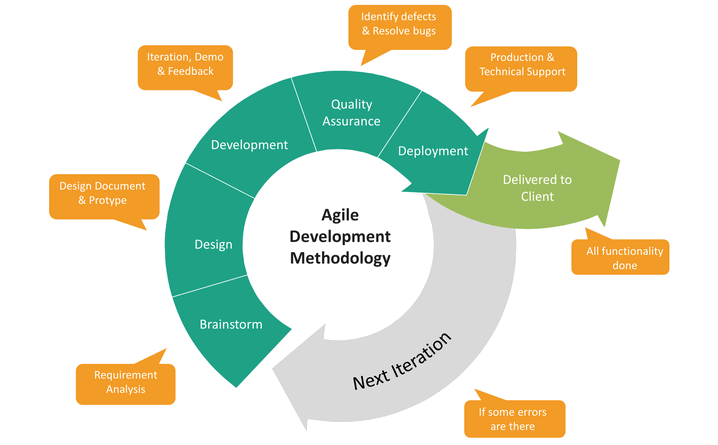
\includegraphics[width=\textwidth,height=0.7\textheight,keepaspectratio]{agile_sdlc.png} \footnote{\url{https://serenagray2451.medium.com/agile-software-development-life-cycle-b3ed0f0f7212}}
\end{frame}
\begin{frame}{Origin}
    \begin{itemize}
        \item Stage at which an Issue \textbf{originated} 
        \item 1 - Planning
        \item 2 - Design
        \item 3 - Implementation
        \item 4 - Validation
        \item 5 - Production
    \end{itemize}
\end{frame}
\begin{frame}{Caught}
    \begin{itemize}
        \item Stage at which an Issue is \textbf{detected}
        \item 1 - Planning
        \item 2 - Design
        \item 3 - Implementation
        \item 4 - Validation
        \item 5 - Production
    \end{itemize}
\end{frame}
\begin{frame}{Volatility}
    $$(Caught - Origin) \times Impact$$
\end{frame}
\end{document}